
%(BEGIN_QUESTION)
% Copyright 2006, Tony R. Kuphaldt, released under the Creative Commons Attribution License (v 1.0)
% This means you may do almost anything with this work of mine, so long as you give me proper credit

En massiv metallkube som er nøyaktig 4 tommer på hver side er neddykket i en åpen beholder fylt med metanol.  Bunnen av kuben ligger 10 tommer under metanoloverflaten:

$$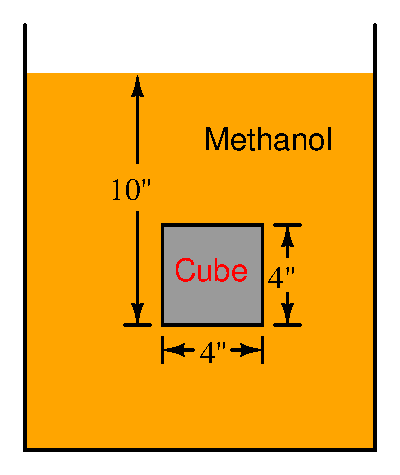
\includegraphics[width=15.5cm]{i00266x01.eps}$$

Basert på beregning av hydrostatisk trykk (i PSI), bestem kraften på hver side av kuben (i pund), samt netto- eller \textit{resultant}-kraften av disse seks kreftene (én kraft på hver side).

Basert på metanoltetthet 49.41 lb/ft$^{3}$, hvor mye veier 64 kubikktommer metanol (en 4" $\times$ 4" $\times$ 4" kube)?

\underbar{file i00266}
%(END_QUESTION)





%(BEGIN_ANSWER)

Kraft opp på kubens bunnflate: 4.575 lb

Kraft ned på kubens toppflate: 2.745 lb

Gjennomsnittlig horisontal kraft på hver av de fire andre flatene: 3.660 lb

\vskip 10pt

Resultantkraft: 1.830 lb (oppover) = vekten av 64 in$^{3}$ metanol ved 49.41 lb/ft$^{3}$.


%(END_ANSWER)





%(BEGIN_NOTES)


%INDEX% Physics, static fluids: buoyancy

%(END_NOTES)
